\chapter{Deseño}
\label{chap:deseño}

Neste capítulo descríbese o deseño da solución, incluíndo a arquitectura do sistema, o modelo de información e de persistencia, os principais fluxos de interacción e a navegación da interface. O obxectivo é presentar as decisións que determinan a organización e o comportamento da aplicación, mentres que a súa materialización no código se explica no Capítulo~\ref{chap:implem}. Os diagramas e fluxos complementarios recóllense no Apéndice~\ref{app:deseno-detallado}.

\section{Arquitectura da solución}

\subsection{Visión xeral do sistema}

A solución segue unha \textbf{arquitectura cliente-servidor} formada por unha aplicación móbil e unha \gls{api} baseada no estilo \gls{rest}. O cliente constitúe o punto de interacción coa persoa usuaria e encárgase do seguimento do tratamento, a persistencia local e as notificacións. A \gls{api} centraliza o procesamento das follas, aplica as regras necesarias para reconstruír a pauta e proporciona acceso aos servizos externos empregados pola solución.

Esta separación evita incorporar no cliente as credenciais e a lóxica de acceso ao servizo de procesamento documental. Ademais, permite modificar ou substituír ese servizo sen alterar o fluxo empregado pola aplicación, sempre que se conserve o contrato de comunicación establecido.

A información clínica e o seguimento das tomas almacénanse localmente nos dispositivos. En consecuencia, a \gls{api} non mantén unha base de datos central cos tratamentos das persoas usuarias e cada petición contén a información necesaria para ser procesada. Esta decisión reduce a cantidade de datos sensibles conservados no servidor e permite consultar a pauta xa gardada sen depender continuamente dunha conexión de rede.

Outro criterio relevante foi non incorporar automaticamente os resultados da extracción ao tratamento activo. Debido a que o proceso documental pode producir datos incompletos ou incorrectos, a pauta pasa sempre por unha fase de revisión e validación antes de ser confirmada.

\subsection{Arquitectura do cliente móbil}

O cliente organízase seguindo o patrón \textit{Model-View-ViewModel} (MVVM). As \textbf{vistas} representan as pantallas e recollen as interaccións da persoa usuaria. Os \textbf{modelos de vista} manteñen o estado asociado ás distintas funcionalidades e coordinan as operacións necesarias. Pola súa parte, os \textbf{modelos} representan a información coa que traballa a aplicación.

A estas capas engádese un conxunto de \textbf{servizos} que encapsulan as operacións que non pertencen directamente á interface, como o acceso á \gls{api}, a persistencia, as notificacións, o almacenamento seguro ou a sincronización. Esta separación permite que as pantallas non necesiten coñecer como se executan esas operacións e facilita probar a lóxica dos modelos de vista de maneira illada.

Os compoñentes visuais reutilizables e os recursos compartidos mantéñense tamén separados das funcionalidades concretas. A correspondencia entre estas responsabilidades e a estrutura de paquetes do proxecto móstrase no Apéndice~\ref{app:deseno-detallado}.

\subsection{Arquitectura da API}

A \gls{api} deseñouse como un servizo sen estado: cada petición é independente e non require unha sesión almacenada no servidor. A súa organización separa catro responsabilidades principais:

\begin{itemize}
    \item os \textbf{puntos de entrada}, que reciben e verifican as peticións;
    \item a \textbf{lóxica interna}, que preprocesa, interpreta, transforma e valida os datos;
    \item os \textbf{esquemas}, que definen os contratos de entrada e saída;
    \item as \textbf{dependencias}, que proporcionan o acceso aos servizos externos.
\end{itemize}

Esta división evita mesturar a comunicación \gls{http} coa lóxica de procesamento e permite substituír as dependencias externas durante as probas. Os contratos \gls{rest} agrúpanse segundo a súa finalidade: extracción das follas, preprocesamento independente, consulta de centros sanitarios, comprobación do estado do servizo e reenvío de notificacións entre dispositivos vinculados.

A Figura~\ref{fig:arquitectura-mvvm-api} mostra conxuntamente a organización do cliente e da \gls{api}, así como a comunicación cos servizos externos.

\begin{figure}[htbp]
    \centering
    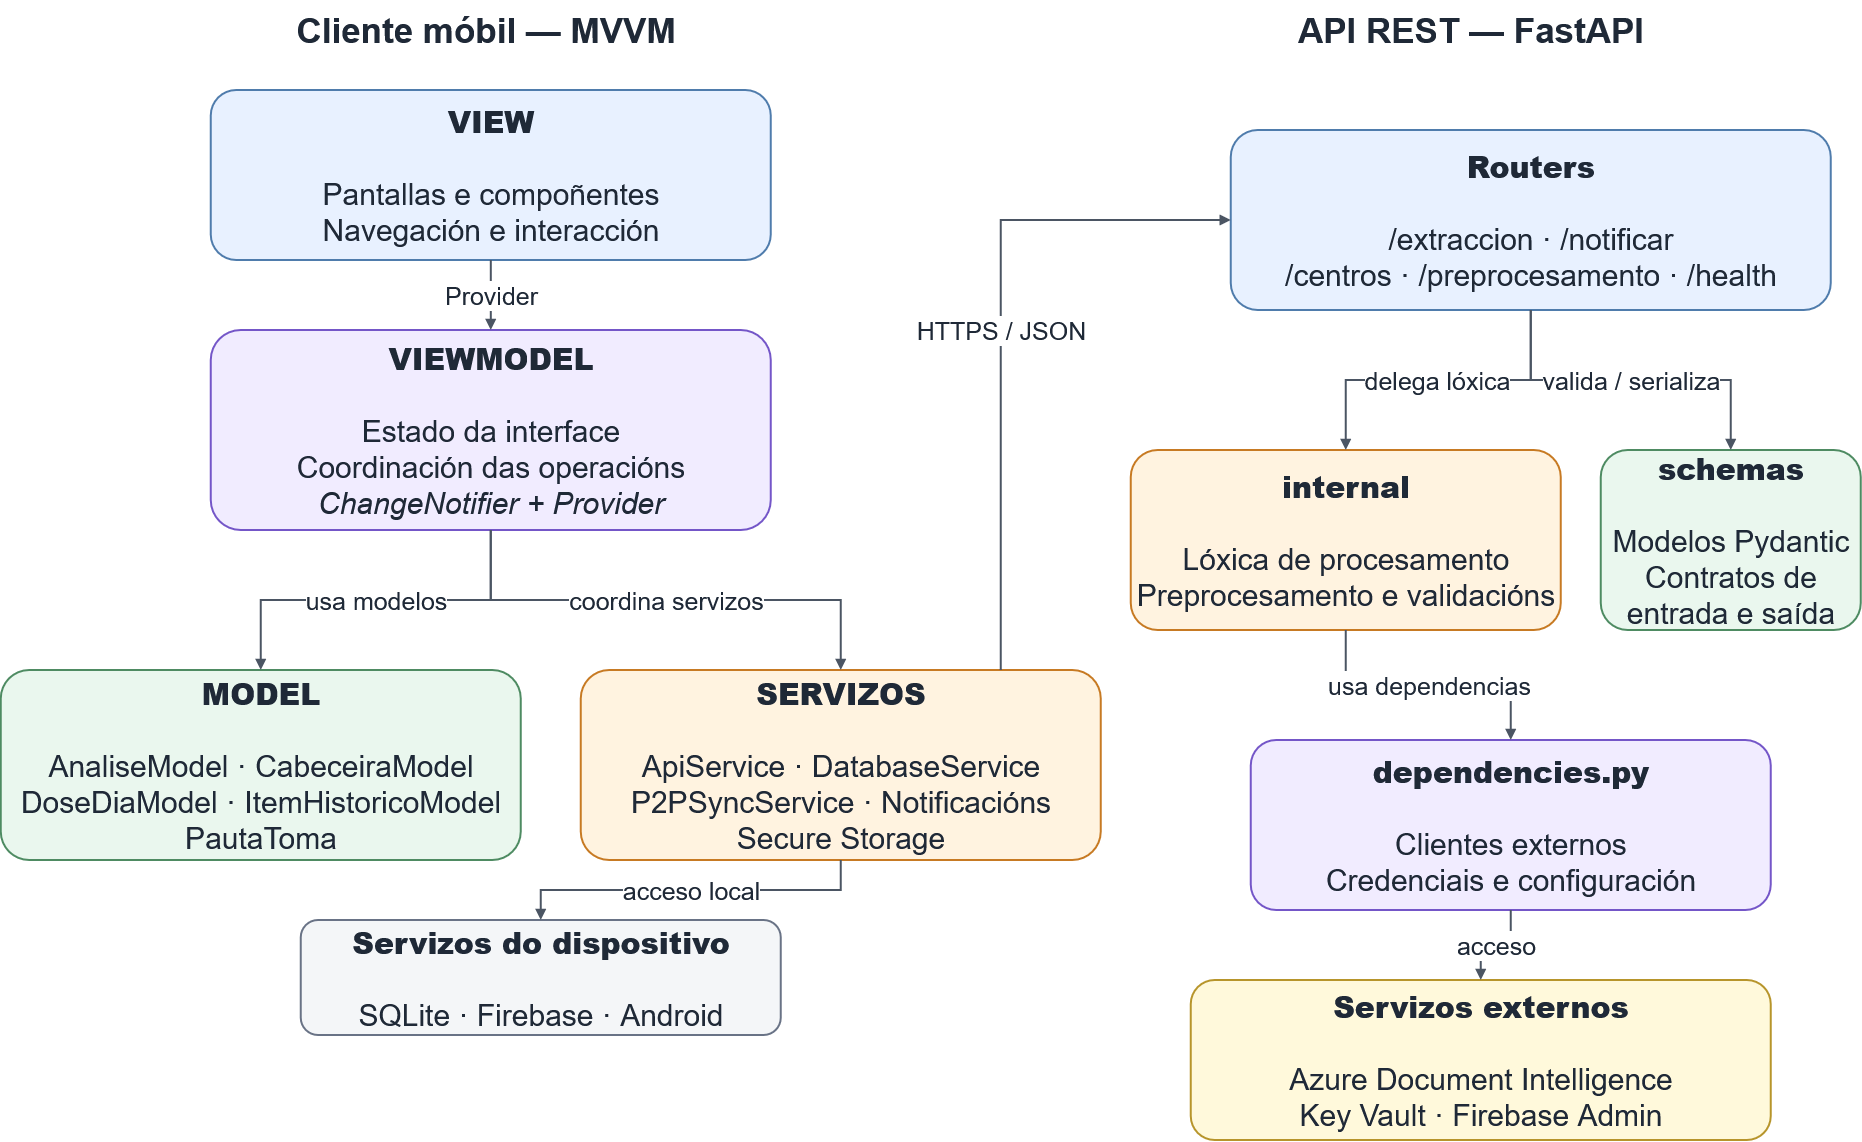
\includegraphics[width=0.92\textwidth]{imaxes/07-Deseño/02_cliente_mvvm_api.drawio(1).png}
    \caption{Arquitectura do cliente móbil e da API.}
    \label{fig:arquitectura-mvvm-api}
\end{figure}

\section{Modelo de información e persistencia}

\subsection{Modelo de información da aplicación}

O modelo principal representa os datos obtidos dunha folla de tratamento e a información necesaria para revisalos e realizar posteriormente o seguimento das tomas.

A entidade principal é a \textbf{análise}, que agrupa tres bloques: a cabeceira, a pauta diaria e o histórico de visitas. A cabeceira reúne datos xerais como a data do informe, o \gls{inr}, o fármaco, a dose semanal, a seguinte visita e o centro sanitario. A pauta diaria está formada polos días de tratamento e indica para cada un deles a data, a dose ou acción correspondente e se se trata dun día de control. O histórico conserva a información das visitas anteriores incluídas no documento.

Sobre esta análise actúa a \textbf{revisión da pauta}. Durante esta etapa poden corrixirse doses e datas, engadir ou eliminar días, modificar a seguinte visita, ordenar a pauta e comprobar a súa consistencia. Deste xeito, diferéncianse os datos propostos pola extracción automática dos datos que a persoa usuaria confirma finalmente.

Unha vez confirmada a pauta, cada dose pasa a formar parte do \textbf{seguimento das tomas}. Ademais da información prescrita, consérvase o estado de cada toma para distinguir se permanece pendente, foi realizada, foi realizada fóra da hora prevista ou non se realizou.

A Figura~\ref{fig:modelo-dominio} mostra os principais elementos deste modelo e as relacións entre eles.

\begin{figure}[htbp]
    \centering
    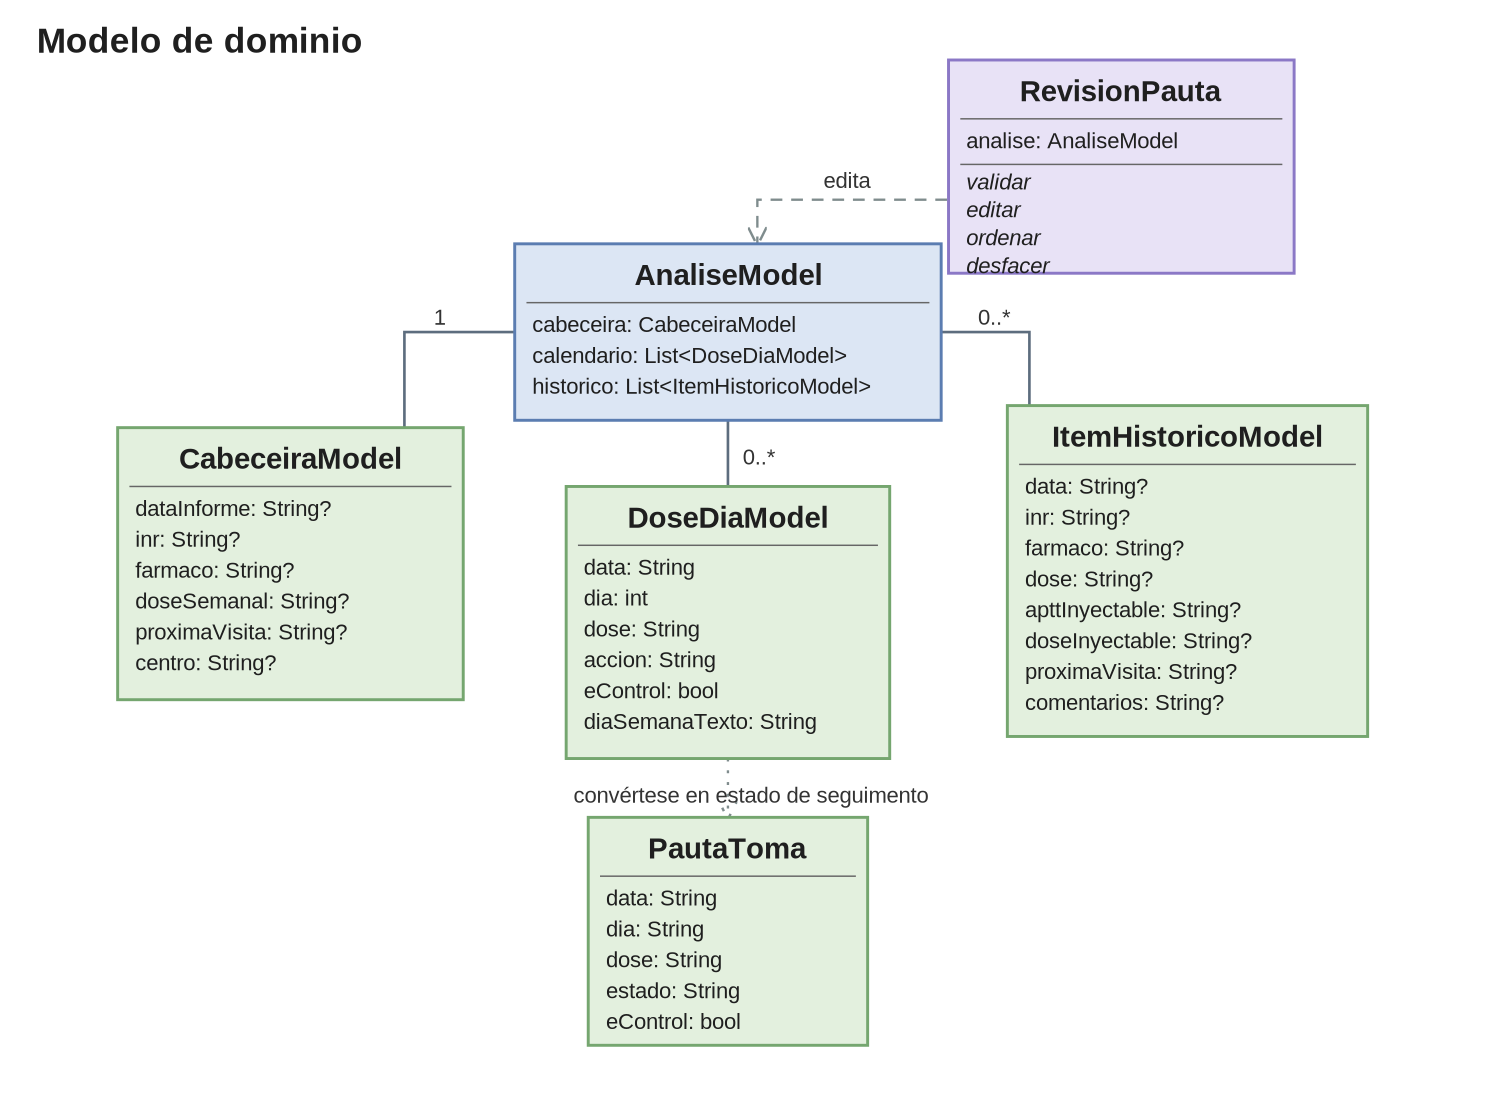
\includegraphics[width=0.8\textwidth]{imaxes/07-Deseño/modelo_dominio_uml_preview.png}
    \caption{Modelo principal de información da aplicación.}
    \label{fig:modelo-dominio}
\end{figure}

\subsection{Modelo de persistencia}

O almacenamento local organízase arredor da pauta vixente, o histórico de visitas e os datos necesarios para a supervisión. A \textbf{pauta vixente} reúne a última folla confirmada e o plan diario, incluíndo o estado das tomas. Cando se confirma unha nova folla, esta substitúe a pauta anterior, polo que só existe un tratamento activo en cada momento.

O \textbf{histórico de visitas} consérvase separado da pauta vixente para permitir consultar a evolución sen mesturala cos datos empregados no seguimento diario. Nos dispositivos das persoas supervisoras almacénanse tamén os \textbf{datos de supervisión}, formados polas persoas vinculadas e pola última información recibida de cada unha delas.

Finalmente, os \textbf{datos de configuración e seguridade}, como o rol, as preferencias e as claves asociadas ás vinculacións, mantéñense separados da base de datos clínica. As claves e os identificadores sensibles gárdanse mediante almacenamento seguro do sistema operativo.

\begin{figure}[htbp]
    \centering
    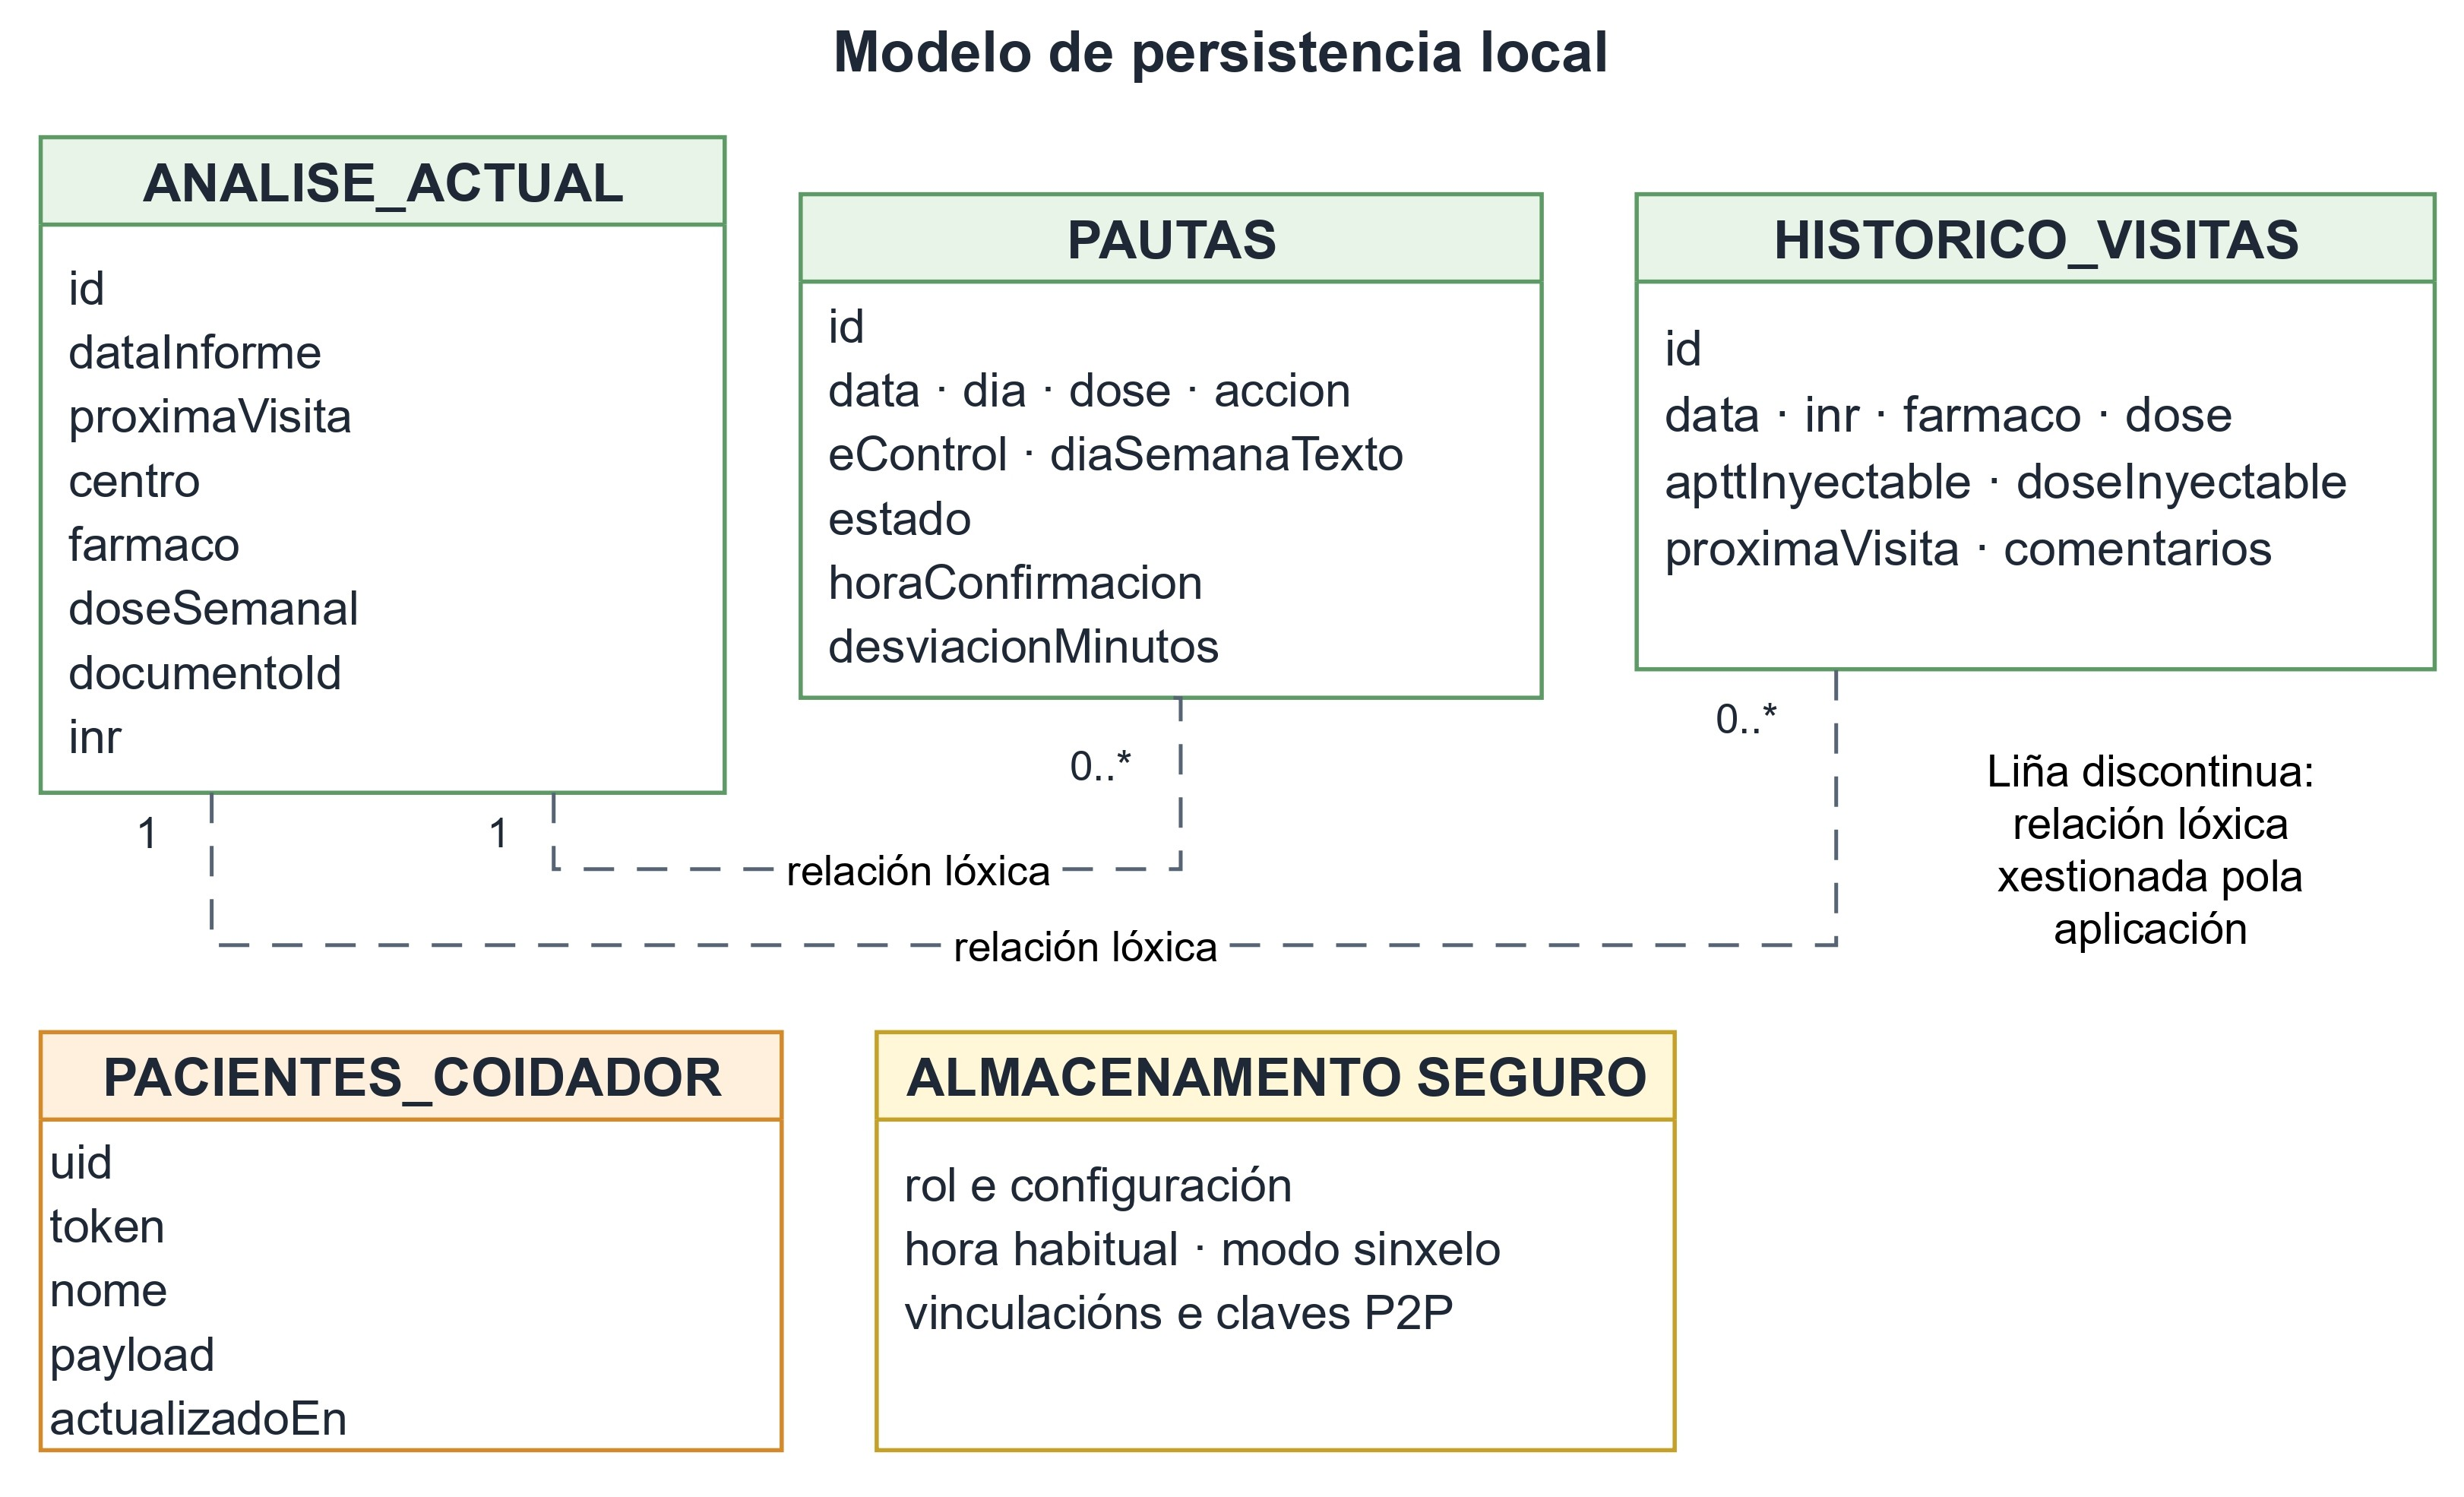
\includegraphics[width=0.8\textwidth]{imaxes/07-Deseño/modelo-persistencia_page-0001.jpg}
    \caption{Modelo entidade--relación da persistencia local.}
    \label{fig:modelo-persistencia}
\end{figure}

\section{Deseño do comportamento}

Nesta sección descríbense os tres fluxos que conectan máis compoñentes da solución: a vinculación entre os dispositivos, o procesamento dunha folla e a sincronización do tratamento.

\subsection{Vinculación entre paciente e supervisor}

A vinculación establécese mediante un código \gls{qr} xerado no dispositivo do paciente. Este código contén un identificador da vinculación, os datos necesarios para localizar o dispositivo e unha clave temporal empregada para protexer o intercambio inicial.

O supervisor escanea o código e utiliza estes datos para iniciar a asociación. Como resposta, envía a súa identificación xunto cunha nova clave compartida que se empregará nas comunicacións posteriores. A información transmítese cifrada coa clave temporal e, unha vez completado o intercambio, ambos os dispositivos dispoñen dos datos necesarios para identificarse e comunicarse de maneira segura.

\begin{figure}[htbp]
    \centering
    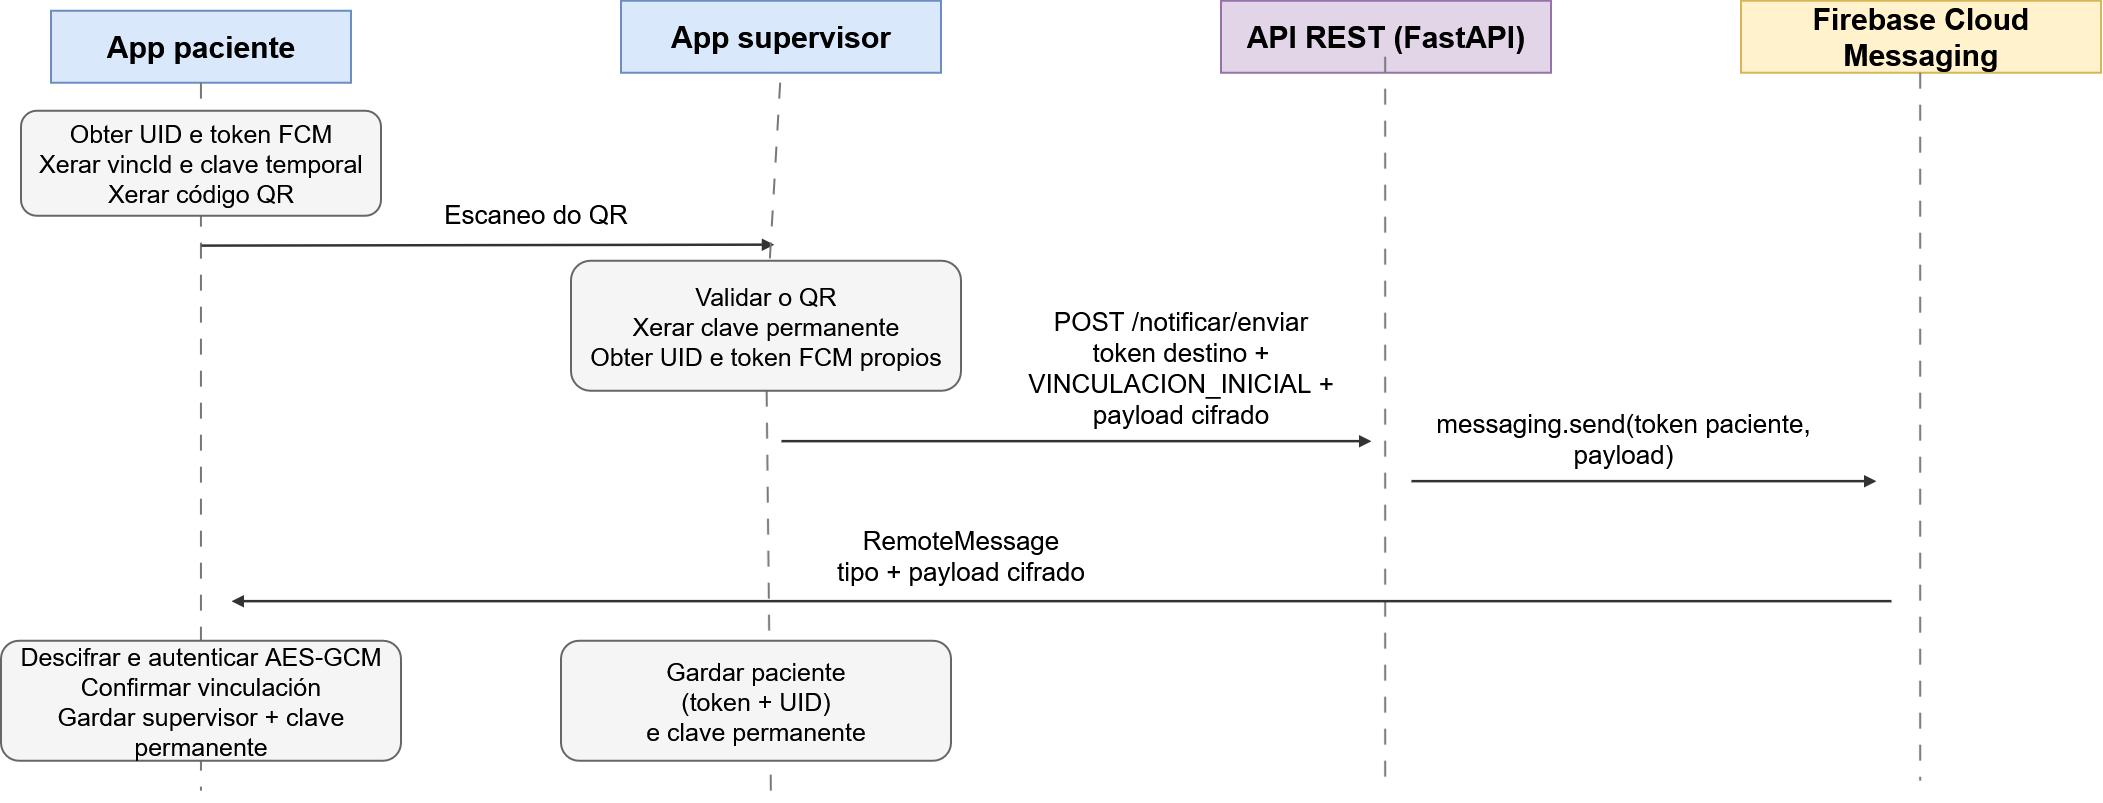
\includegraphics[width=0.9\textwidth]{imaxes/07-Deseño/secuencia_vinculacion_UML.drawio.png}
    \caption{Fluxo de vinculación entre paciente e supervisor.}
    \label{fig:fluxo-vinculacion}
\end{figure}

\subsection{Procesamento dunha folla de tratamento}

O fluxo comeza cando a persoa usuaria selecciona ou captura unha folla desde a aplicación. O documento envíase á \gls{api}, que comproba o formato, realiza o preprocesamento cando é necesario e solicita a extracción ao servizo documental.

A partir do resultado, a \gls{api} normaliza os campos, reconstrúe a pauta diaria e realiza as validacións definidas antes de devolver unha resposta. No cliente, os datos móstranse nunha pantalla de revisión e só pasan a formar parte da pauta activa despois da confirmación. Se a extracción non supera as comprobacións mínimas, o fluxo interrómpese e solicítase unha nova captura.

\begin{figure}[htbp]
    \centering
    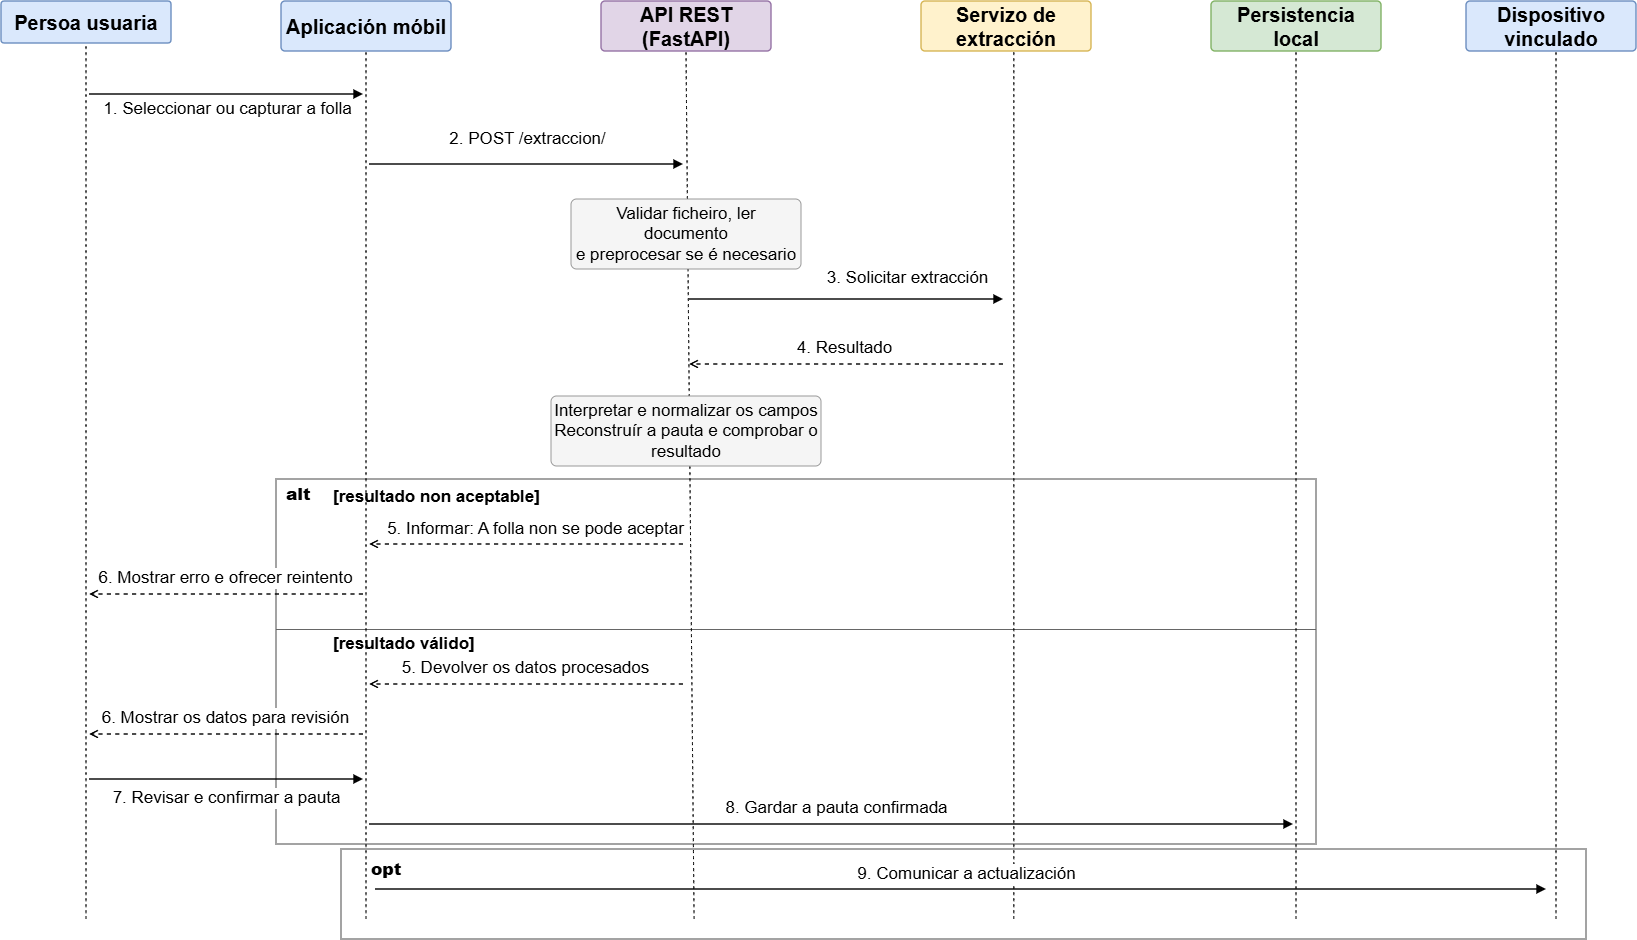
\includegraphics[width=0.9\textwidth]{imaxes/07-Deseño/secuencia_procesamento_UML.drawio.png}
    \caption{Fluxo de procesamento dunha folla de tratamento.}
    \label{fig:fluxo-procesamento}
\end{figure}

\subsection{Sincronización entre dispositivos}

Cando se produce un cambio que debe compartirse, como a confirmación dunha toma ou a incorporación dunha nova folla, o dispositivo de orixe prepara a información e cífraa empregando a clave acordada durante a vinculación. A mensaxe cifrada envíase á \gls{api}, que actúa como intermediaria e a reenvía mediante o servizo de mensaxería.

O dispositivo de destino autentica e descifra a mensaxe antes de actualizar a súa información local. Deste xeito, a \gls{api} participa no transporte sen necesitar interpretar nin almacenar o contido clínico intercambiado.

\begin{figure}[htbp]
    \centering
    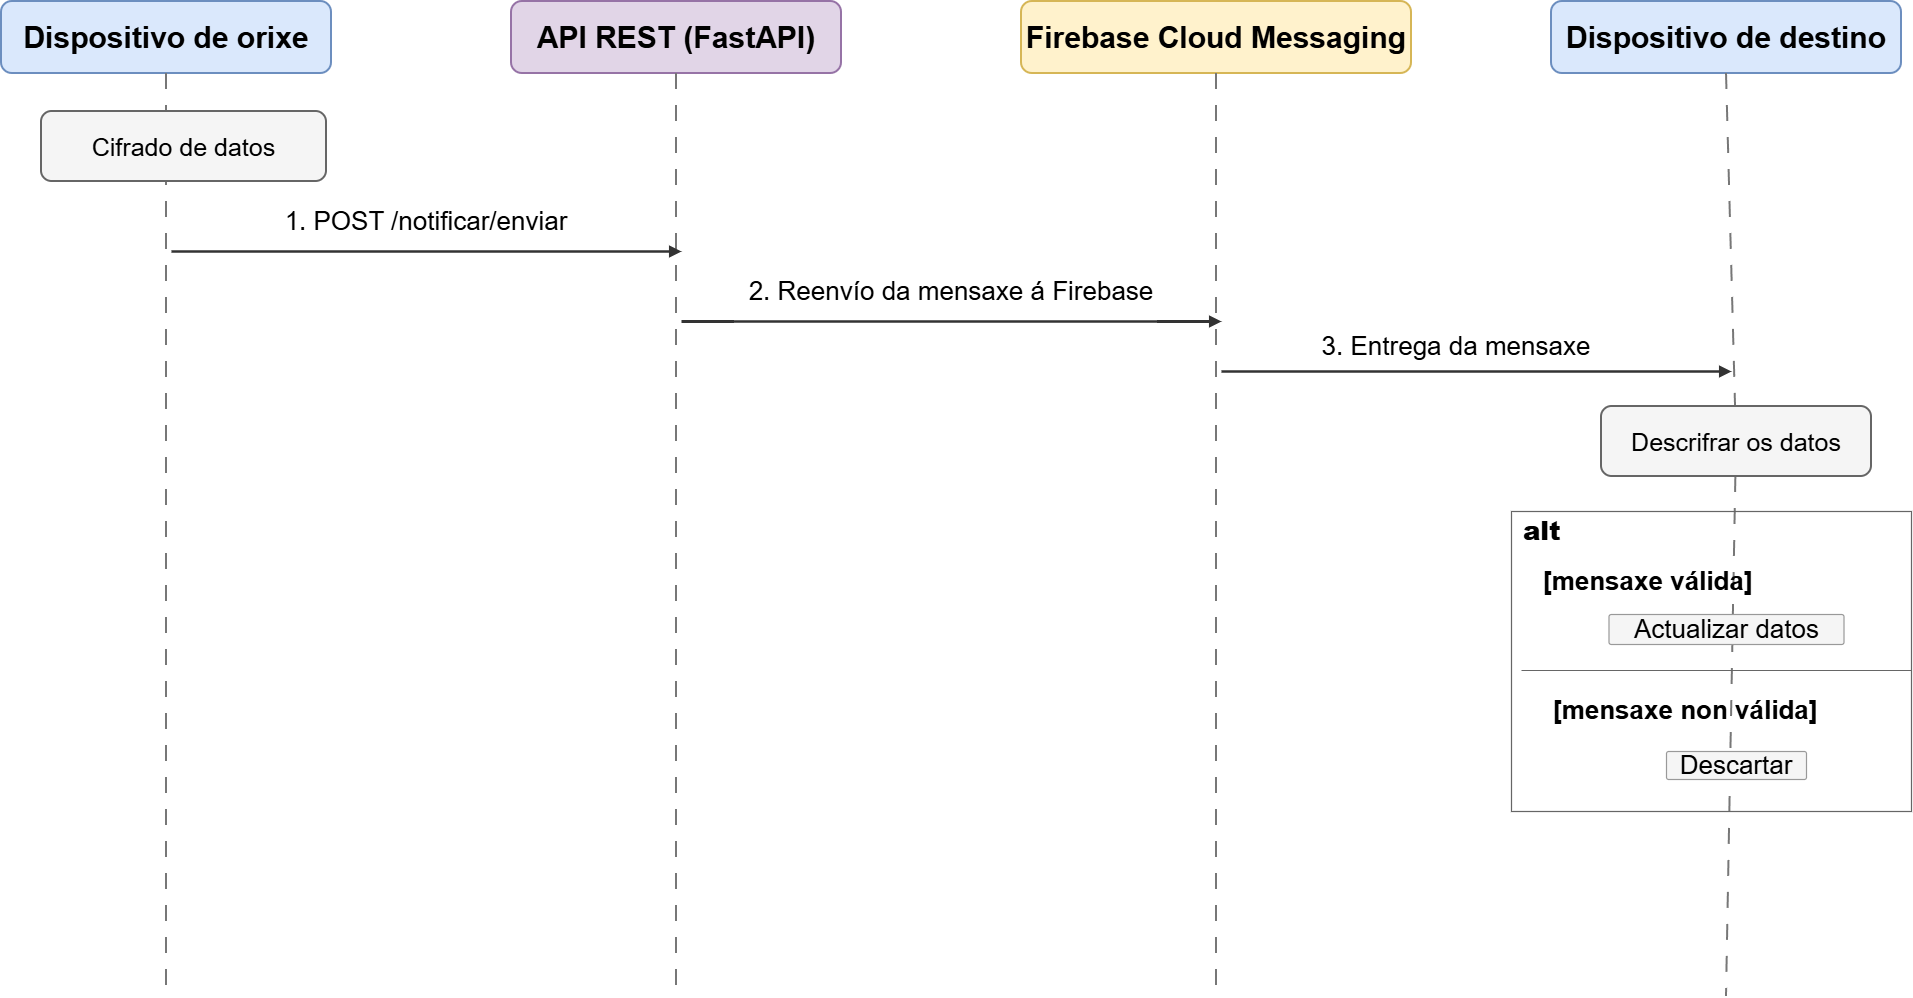
\includegraphics[width=0.9\textwidth]{imaxes/07-Deseño/secuencia_sincronizacion_UML.drawio.png}
    \caption{Fluxo de sincronización entre dispositivos vinculados.}
    \label{fig:fluxo-sincronizacion}
\end{figure}

\section{Deseño da navegación e da interface}

\subsection{Fluxo de navegación}

O primeiro acceso comeza coa selección do rol, decisión que determina as funcionalidades e o percorrido posterior. No caso do \textbf{paciente}, o fluxo inclúe a xeración do código \gls{qr}, a configuración dos permisos de dixitalización e a introdución de datos como o nome e a hora habitual da toma. A pantalla principal permite acceder á pauta, ao calendario, ao progreso, á incorporación dunha nova folla e aos axustes.

No caso da \textbf{persoa supervisora}, o proceso inicial emprega a cámara para escanear o código xerado polo paciente. Tras completar a vinculación, a pantalla principal mostra as persoas supervisadas. Ao seleccionar unha delas accédese ao seu tratamento, ao estado das tomas e ás operacións dispoñibles para a súa supervisión.

A separación por roles evita mostrar opcións que non corresponden á responsabilidade seleccionada e simplifica os percorridos máis habituais de cada tipo de persoa usuaria.

\begin{figure}[htbp]
    \centering
    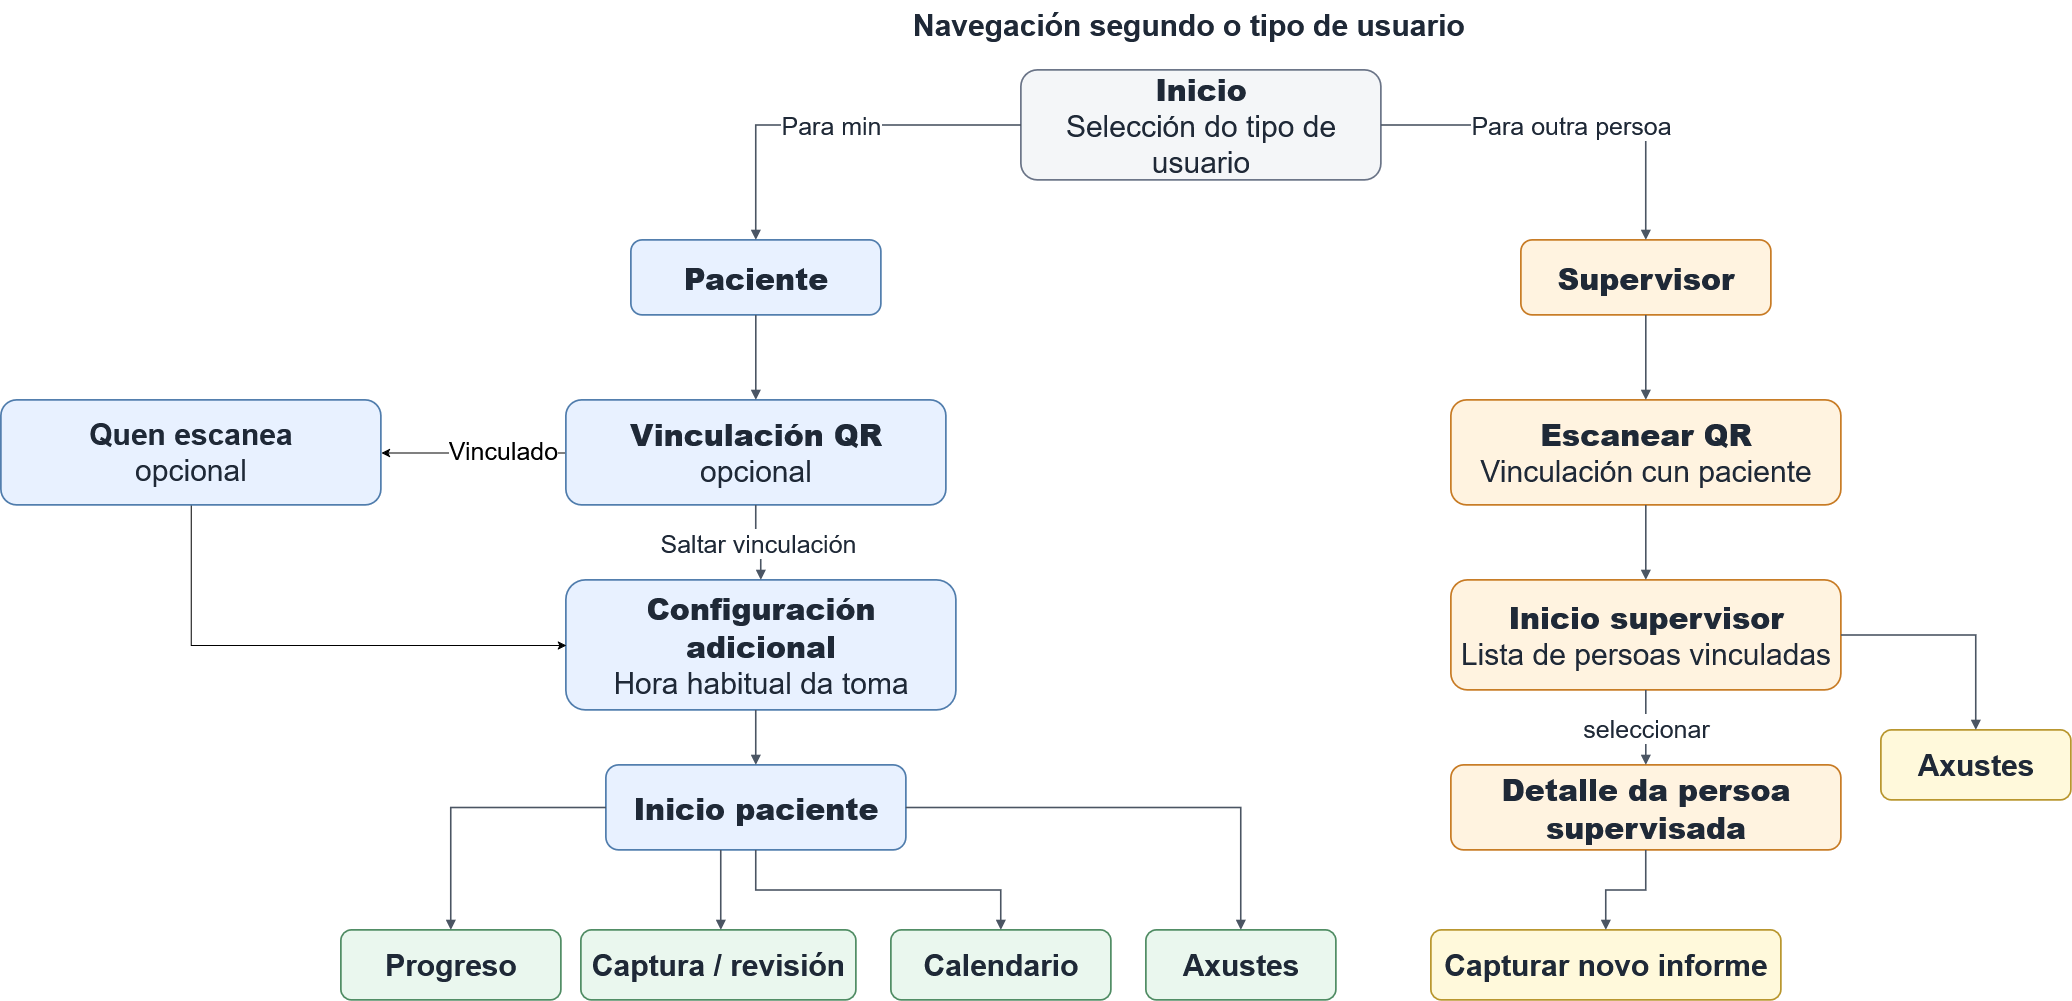
\includegraphics[width=\textwidth]{imaxes/07-Deseño/diagrama fluxo.drawio.png}
    \caption{Fluxo de navegación das pantallas segundo o tipo de usuario.}
    \label{fig:navegacion-pantallas}
\end{figure}

\subsection{Wireframes da interface}

Antes da implementación elaboráronse en Figma distintos wireframes para definir a distribución da información e comprobar os principais percorridos. Estes deseños serviron como referencia inicial, aínda que algúns elementos se adaptaron durante o desenvolvemento ao comprobar o seu funcionamento en dispositivos reais.

Na Figura~\ref{fig:wireframes-principais} móstranse os wireframes máis representativos: selección do rol, pantalla principal do paciente, incorporación dunha folla e pantalla principal da persoa supervisora. O conxunto completo, incluíndo as pantallas de vinculación, revisión, calendario, progreso e configuración, recóllese no Apéndice~\ref{app:wireframes}.

\begin{figure}[htbp]
    \centering
    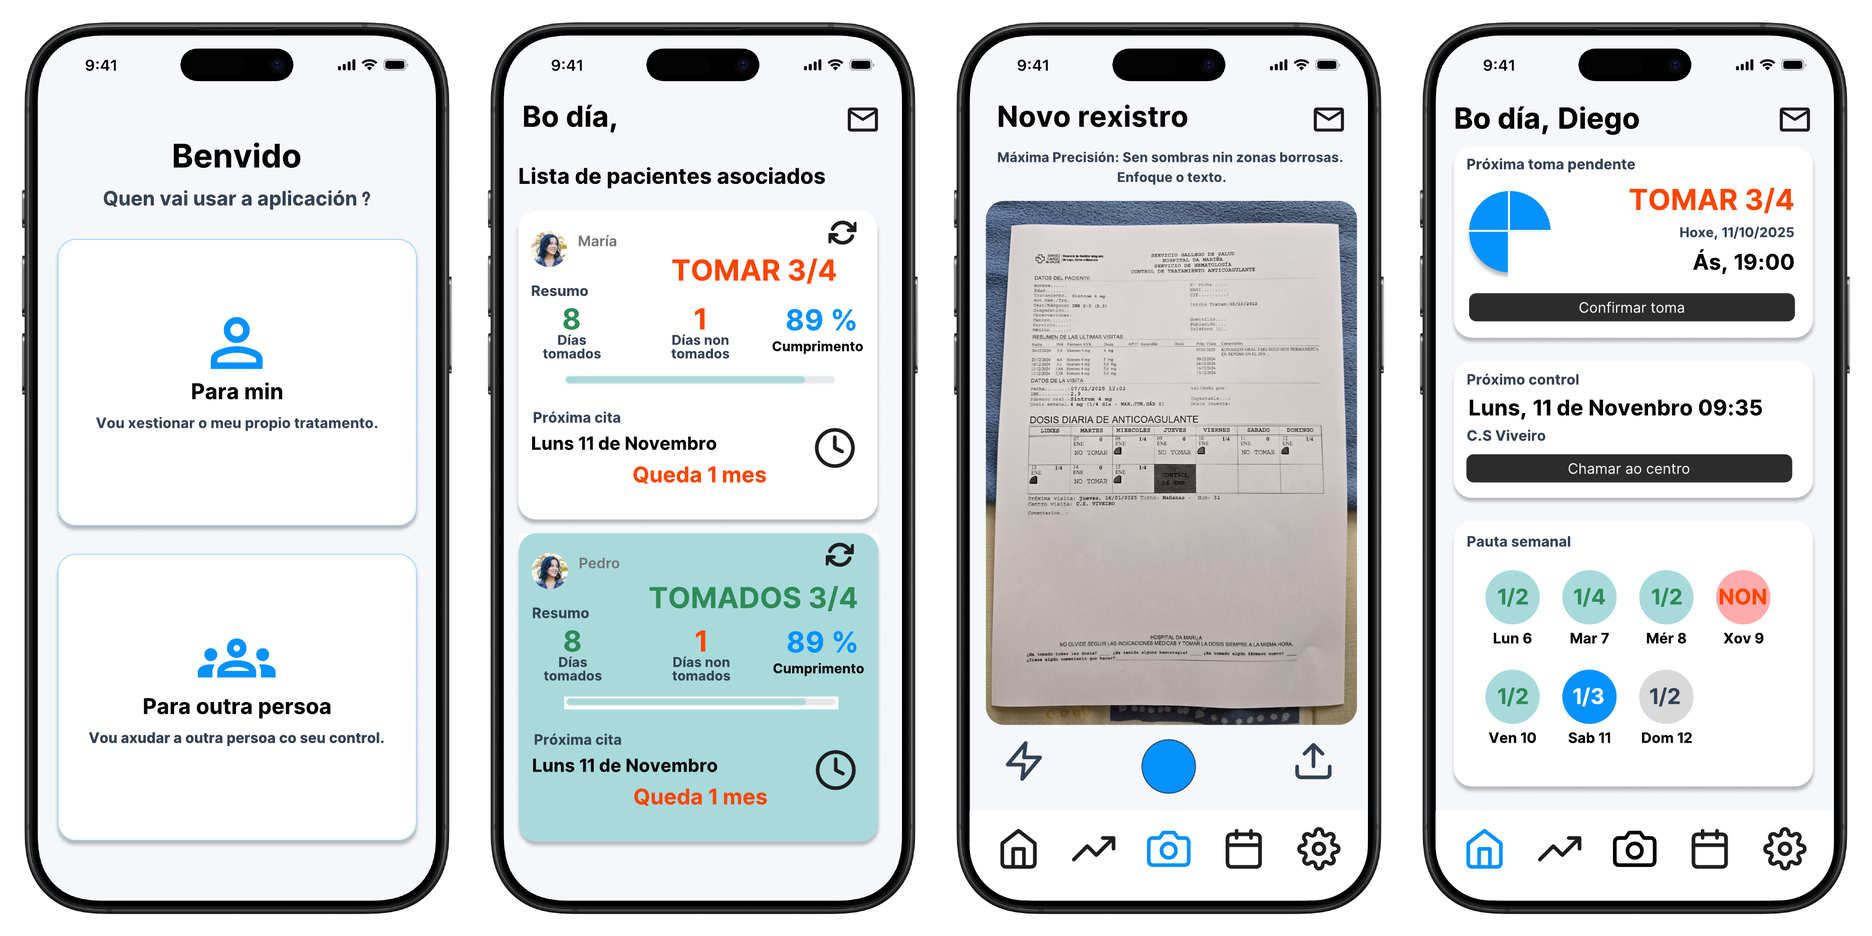
\includegraphics[width=0.90\textwidth]{imaxes/07-Deseño/wireframes_principais.png}
    \caption{Wireframes representativos da interface da aplicación.}
    \label{fig:wireframes-principais}
\end{figure}
